\documentclass{report}

\usepackage[utf8]{inputenc} % Charakter-Kodierung
\usepackage[german]{babel} % Sprache

\usepackage[table,xcdraw]{xcolor} % Tabellen Farben
\usepackage{tabularx} % Dynamische Tabellenbreite
\usepackage{tcolorbox} % Graue Boxen
\usepackage{hyperref} % url Umgebung
\usepackage{todonotes} % Notizen
\usepackage{natbib} % Bibliographie
\usepackage{fancyhdr} % Header und Footer
\usepackage{multirow} % Multizeile
\usepackage{geometry} % Page layout
\usepackage{color} % Text Farben
\usepackage{enumitem}
\usepackage{array}

% Page layout
\geometry{
	bottom=3.5cm,
	headheight=180pt
}

% Nummerierung der ersten Seiten verhindern
\pagenumbering{gobble}

% Bibstyle
\bibliographystyle{plain}

% Header / Footer
\fancypagestyle{plain}{
	\fancyhf{}% Clear header/footer
	\fancyhead[R]{\includegraphics[width=4cm]{img/cau-logo-2017}} % Rechter header
	\fancyhead[L]{\leftmark} % Linker header
	\fancyfoot[R]{\thepage} % Rechter footer
	\fancyfoot[L]{\includegraphics[width=1cm]{img/se-logo}} % Linker footer
}
\pagestyle{plain}

\renewcommand{\headrulewidth}{0.5pt} % Unnötige Informationen der Kapitelangabe
\renewcommand{\footrulewidth}{0.2pt} % entfernen
\renewcommand{\chaptermark}[1]{\markboth{{#1}}{}}




% Zahlen für Fußnoten
\renewcommand{\thefootnote}{\arabic{footnote}}
\renewcommand{\thempfootnote}{\arabic{mpfootnote}}

%%%%% Ausfüllen %%%%%

% Gruppenname
\newcommand{\gruppenname}{Gruppe X}

% Projektname
\newcommand{\projektname}{Projektname}

% Semester
\newcommand{\semester}{SoSe17}



% Titelseite

\title{
	\vspace*{-3cm}
	Entwurfsdokumentation\\
	\projektname\\
	-\\
	\color{gray}
	Softwareprojekt \semester\\
	\gruppenname\\
	\vspace*{5mm}
	
\includegraphics[width=\textwidth]{img/logo}
}

\author{
	\begin{tabular}{r l@{\hspace{8\tabcolsep}} r}
		Vorname1 & Nachname1 & \multirow{8}{*}{ \includegraphics{img/se-logo} } \\
		Vorname2 & Nachname2 \\
		Vorname3 & Nachname3 \\
		Vorname4 & Nachname4 \\
		Vorname5 & Nachname5 \\
		Vorname6 & Nachname6 \\
		Vorname7 & Nachname7 \\
		Vorname8 & Nachname8 \\
	 \end{tabular}
}

\date{\today}





% Dokument

\begin{document}
	\maketitle

	%%%% Bitte löschen oder auskommentieren %%%%
	%%%%%%%%% Dient nur als Hilfe %%%%%%%%%%

	\chapter*{Tipps und Hilfen}\label{chp:tipps}
	\vspace*{-1cm}
	\begin{tcolorbox}
		\textbf{Information:} Dieses Kapitel und alle folgenden grauen Boxen dienen als Hilfestellungen und sollen im fertigen Dokument nicht enthalten sein.
		%
		\\\\
		%
		Zur Versionsverwaltung während des Softwareprojekts muss \textit{Git} genutzt werden.
		Git führt Textdokumente mit unterschiedlichen Zeilenbearbeitungen automatisch zusammen.
		Wir empfehlen den Einsatz von \LaTeX~für alle Textdokumente.
		Um das Auto-Merging zu unterstützen, sollte nach jedem Satzende eine neue Zeile im Quelltext begonnen werden.
		Die .tex-Datei dieser PDF verdeutlicht dies.
		Erkennt Git, dass eine gleiche Zeile bearbeitet wurde, wird ein Konflikt auftreten.
		Dieser kann in der entsprechenden Datei von Hand mittels eines Texteditors behoben werden.
		%
		\\\\
		%
		Fußnoten\footnote{\url{https://www.se.informatik.uni-kiel.de/en}} werden für Homepages genutzt.
		Zitierungen können mittels eines \textit{cite}-Befehls gesetzt, z.B. \textit{citep}~\citep{Shaw2003WritingGoodSoftwareEngineeringesearchPapersMinitutorial}.
		%
		\\\\
		%
		Tipps zur UML-Modellierung können im SE-Wiki\footnote{\url{https://git.informatik.uni-kiel.de/ag-se/teaching-public/wikis/home}} nachgelesen werden.
		Achtet darauf, dass eure Diagramme stets lesbar (Vektor-Grafiken!) und gut strukturiert sind.
		Oftmals ist es sinnvoll ein bis zwei Sätze zusätzlich für Diagrammelemente zu formulieren.
		So können Missverständnisse ausgeschlossen werden, was einen Einfluss auf die Korrektur haben kann.
		Diagramme für unwichtige Tätigkeiten (z.B. Login / Logout, User erstellen / löschen, Passwort ändern etc.) sind nicht erforderlich.
	\end{tcolorbox}

	\todo[inline]{So kann eine TODO-Notiz erzeugt werden}

	\begin{figure}[h]
		\centering
		\missingfigure{So kann eine Placeholder-Grafik beispielsweise in den Text eingefügt werden.}
		\caption{Beschreibung}
		\label{fig:x}
	\end{figure}

	%%%%%%%%%%%%%%%%%%%%%%%%%%%%%%

	\tableofcontents

	\chapter{Einleitung}\label{chp:einleitung}
	\pagenumbering{arabic} % Nummerierung starten
	\thispagestyle{fancy}
	\section{Dokumentaufbau}\label{sec:dokumentaufbau}
\begin{tcolorbox}
	Inhalt und Struktur des vorliegenden Dokuments skizzieren (Fließtext).
\end{tcolorbox}

\section{Zweckbestimmung}\label{sec:zweckbestimmung}
\begin{tcolorbox}
	Zweck des ganzen Systems beschreiben (Fließtext).
\end{tcolorbox}

\section{Entwicklungsumgebung}\label{sec:entwicklungsumgebung}
\begin{tcolorbox}
	Oftmals treten neue Entwickler einem Projekt bei oder ein Entwicklungs-Rechner muss ersetzt werden.
	Daher sollen hier nennenswerte und grundlegende Frameworks, Bibliotheken, Tools und Sprachen notiert werden.
	Tabelle X stellt eine beispielhafte Umsetzung dar.
	Eine Unterteilung in Komponenten ist sinnvoll.
\end{tcolorbox}

\begin{table}[h]
	\centering
	\begin{tabularx}{\textwidth}{l l X}
		\rowcolor[HTML]{C0C0C0} 
		\textbf{Software} & \textbf{Version} & \textbf{URL} \\
		Java Development Kit & 8u144 & \url{http://www.oracle.com/technetwork/java/javase/downloads/index.html} \\
		\rowcolor[HTML]{E7E7E7} 
		Software X & Version X & URL X \\
		Software X & Version X & URL X \\
		\rowcolor[HTML]{E7E7E7} 
		Software X & Version X & URL X \\
		Software X & Version X & URL X \\
		\rowcolor[HTML]{E7E7E7} 
		Software X & Version X & URL X \\
		Software X & Version X & URL X \\
	\end{tabularx}
	\caption{Enwicklungsumgebung}
	\label{table:entwicklungsumgebung}
\end{table}

	\chapter{Komponentendiagramme}\label{chp:komponentendiagramme}
	\thispagestyle{fancy}
	\begin{figure}[h]
	\centering
	\missingfigure{Komponentendiagramm}
	\caption{Komponentendiagramm - A}
	\label{fig:komponentendiagramm-a}
\end{figure}

Die Serverkomponente bzw. das Backend beschreibt die internen Vorgänge der Software.
Diese Komponente ist über drei verschiedene Schnittstellen, die die unterschiedlichen
Benutzerrechte repräsentieren erreichber.
In der Komponente Benutzerverwaltung werden die Daten der Benutzer aus der Datenbank ausgelesen und verarbeitet.
Dadurch kann die Benutzerverwaltung eine Authentifizierungsschnittstelle für die anderen Subkomponenten bereit stellen.
Zudem kann die Rechteverwaltung manipuliert werden, falls über die Verwalten-Schnittstelle zugegriffen wird.
Die Komponente Diensteverwaltung liest die Daten der Dienste aus der Datenbank aus und verarbeitet diese.
Von außen kann auf die Diensteverwaltung durch die Schnittstellen Bearbeiten und Einsehen zugegriffen werden.
Die Schnittstelle bearbeiten ist nur für Administratoren über die Schnittstelle Verwalten zugänglich.
Es bei jedem Zugriff die Rechte des zugreifenden Benutzers durch die Schnittstelle Auth der Benutzerverwaltung überprüft.
Die Komponente Kompositionsverwaltung stellt die benötigten Funktionen für das Bearbeiten und Einsehen von Kompositionen zur Verfügung und bekommt die Daten dafür von den Komponenten Datenbank und Diensteverwaltung.
Das Bearbeiten von Kompositionen ist nur über die Schnittstellen Bearbeiten und Verwalten möglich, das Einsehen auch über das Einsehen-Interface.
Die Komponente Datenbank speichert alle nötigen Daten für die Komponenten Benutzer-, Dienste- und Kompositionsverwaltung und stellt diese bei Bedarf zur Verfügung.
Zusätzlich kann man über die Einsehen-Schnittstelle auch direkt auf die Authentifizierung zugreifen um ein initiales regestrieren und den Login zu ermöglichen.

Die Komponente Web mit der Subkomponente View Verwaltung ist für die Darstellung in der Webapplikation zuständig.
Da über die Weboberfläche sowohl verwaltet, bearbeitet und eigesehen werden können soll, ist die Web-Komponete auch mit all diesen Schnittstellen verbunden.
Die Komponente App mit der Subkomponente View dient zur Darstellung der angefragten Daten in der App.
In der App können nur Kompositionen eingesehen werden, daher ist diese nur mit der Einsehen-Schnittstelle verbunden.


	\chapter{Verteilungsdiagramm}\label{chp:verteilungsdiagramm}
	\thispagestyle{fancy}
	\begin{figure}[h]
	\centering
	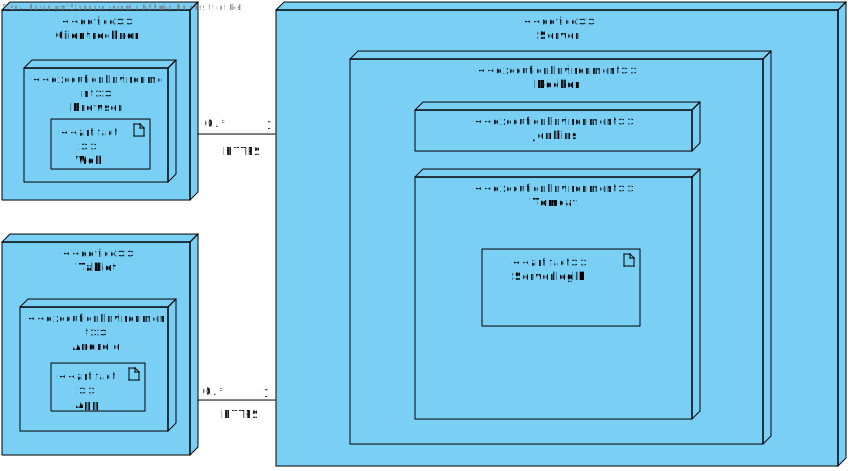
\includegraphics[width=\textwidth]{img/Diagramme/Verteilung}		
	\caption{Verteilungsdiagramm}
	\label{fig:verteilungsdiagramm}
\end{figure}
\noindent
Die App-Komponente läuft auf einem Tablet Android 6.0 oder höher, während 
die Web-Komponente  in den Browsern auf dem Rechnern des Nutzers läuft.
Die Geschäftslogik in der Komponente Serverlogik wird auf einem physikalischen Server ausgeführt, auf dem in einem Docker-Image neben Apache Tomcat auch Jenkins betrieben wird.
Sowohl die Clientrechner als auch die Tablets sind mit dem Server über HTTPS verbunden.

\newpage
\section{REST Schnitstelle}
\begin{table}[htbp]
\centering
\begin{tabularx}{\linewidth+20pt}{|X|l|X|}
\hline
\rowcolor[HTML]{C0C0C0}
\textbf{Aktion} & \textbf{HTTP Methode} & \textbf{Endpunkt}\\
\rowcolor[HTML]{E7E7E7}
createService(s) & POST & /services\\
editService & PUT & /services/\{service\(_{\text{id}}\)\}\\
\rowcolor[HTML]{E7E7E7}
getServices & GET & /services\\
getServiceDetails & GET & /services/\{service\(_{\text{id}}\)\}\\
\rowcolor[HTML]{E7E7E7}
deleteService & DELETE & /services/\{service\(_{\text{id}}\)\}\\
\hline
checkCompatibility & GET & /services/\{user\(_{\text{id}}\)\(_{\text{1}}\)\}/\{user\(_{\text{id}}\)\(_{\text{2}}\)\}\\
\hline
\rowcolor[HTML]{E7E7E7}
getCompositions & GET & /compositions\\
getCompositionDetail & GET & /compositions/\{comp\(_{\text{id}}\)\}\\
\rowcolor[HTML]{E7E7E7}
createComposition & POST & /compositions\\
editComposition & PUT & /compositions/\{comp\(_{\text{id}}\)\}\\
\rowcolor[HTML]{E7E7E7}
\hline
getUserPermissions & GET & /compositions/\{comp\(_{\text{id}}\)\}/users\\
createUserPermission & POST & /compositions/\{comp\(_{\text{id}}\)\}/users/\{email\}\\
\rowcolor[HTML]{E7E7E7}
editUserPermission & PUT & /compositions/\{comp\(_{\text{id}}\)\}/users/\{email\}\\
deleteUserPermission & DELETE & /compositions/\{comp\(_{\text{id}}\)\}/users/\{user\(_{\text{id}}\)\}\\
\rowcolor[HTML]{E7E7E7}
\hline
getUsers & GET & /users\\
getUserDetails & GET & /users/\{user\(_{\text{id}}\)\}\\
\rowcolor[HTML]{E7E7E7}
editUser & PUT & /users/\{user\(_{\text{id}}\)\}\\
register & POST & /users\\
\hline
\end{tabularx}
\caption{Art der Anfrage und zu kontaktierender Endpunkt der API}
\end{table}
\label{sec:org9044419}
\begin{table}[htbp]
\centering
\begin{tabularx}{\linewidth+20pt}{|X|l|X|}
\hline
\rowcolor[HTML]{C0C0C0}
\textbf{Aktion} & \textbf{Inhalt der Anfrage} & \textbf{erwartete Antwort} \\
\rowcolor[HTML]{E7E7E7}
createService(s) & List of services & 201 - CREATED\\
editService & single service & 200 - OK\\
\rowcolor[HTML]{E7E7E7}
getServices & query: string & 200 - OK + List of \emph{Service}\\
getServiceDetails & - & 200 - OK + \emph{Service}\\
\rowcolor[HTML]{E7E7E7}
deleteService & - & 200 - OK\\
\hline
checkCompatibility & - & 200 - OK + \emph{CompatibilityAnswer}\\
\hline
\rowcolor[HTML]{E7E7E7}
getCompositions & - & 200 - OK + List of \emph{SimpleComp}\\
getCompositionDetail & - & 200 - OK + \emph{DetailComp}\\
\rowcolor[HTML]{E7E7E7}
createComposition & name: string & 201 - CREATED\\
editComposition & \emph{Composition Object} & 200 - OK\\
\rowcolor[HTML]{E7E7E7}
\hline
getUserPermissions & \emph{userAuthorizations} & 200 - OK + List of \emph{SimpleUser}\\
createUserPermission & \emph{userPermission Object} & 201 - CREATED\\
\rowcolor[HTML]{E7E7E7}
editUserPermission & \emph{userPermission Object} & 200 - OK\\
deleteUserPermission & - & 200 - OK\\
\rowcolor[HTML]{E7E7E7}
\hline
getUsers & query: string & 200 - OK + List of \emph{SimpleUser}\\
getUserDetails & - & 200 - OK + \emph{DetailUser}\\
\rowcolor[HTML]{E7E7E7}
editUser & \emph{Detail User} & 200 - OK\\
register & \emph{User} & 201 - CREATED\\
\hline
\end{tabularx}
\caption{Argumente und erwartete Rückgabe eine API Anfrage}
\end{table}

	\chapter{Klassendiagramme}\label{chp:klassendiagramme}
	\thispagestyle{fancy}
	\begin{figure}[h]
	\centering
	\missingfigure{Klassendiagramm}		
	\caption{Klassendiagramm - A}
	\label{fig:klassendiagramm-a}
\end{figure}

\begin{table}[h]
	\centering
	\begin{tabularx}{\textwidth}{X X}
		\rowcolor[HTML]{C0C0C0} 
		\textbf{Klassenname} & \textbf{Aufgabe} \\
		Klasse A & Aufgabe A \\
		\rowcolor[HTML]{E7E7E7} 
		Klasse B & Aufgabe B \\
		Klasse C & Aufgabe C \\
		\rowcolor[HTML]{E7E7E7} 
		Klasse D & Aufgabe D \\
		Klasse E & Aufgabe E \\
		\rowcolor[HTML]{E7E7E7} 
		Klasse F & Aufgabe F \\
		Klasse G & Aufgabe G
	\end{tabularx}
	\caption{Klassenbeschreibung - A}
	\label{table:klassenbeschreibung-a}
\end{table}

\begin{tcolorbox}
Teilt eure Klassendiagramme bitte auf und baut \textbf{kein} einzelnes riesiges Diagramm.
Getter und Setter Methoden müssen hier nicht modelliert werden.
Sie sollten aber der klassischen Namenskonvention folgen, um die Nutzung in Sequenzdiagrammen zu ermöglichen.
\\\\
Auf jedes Diagramm folgt eine Tabelle, in der die Aufgabe \textbf{jeder} Klasse beschrieben wird.
\end{tcolorbox}

\section*{Klassendiagramm zur Android-App}

\begin{figure}[h]
	\centering
	\includegraphics[width=\textwidth]{Klassendiagramm_App/Class_Diagram1}
	\caption{Klassendiagramm - App}
	\label{fig:klassendiagramm-a}
\end{figure}

\begin{table}[h]
	\centering
	\begin{tabularx}{\textwidth}{X X}
		\rowcolor[HTML]{C0C0C0} 
		\textbf{Klassenname} & \textbf{Aufgabe} \\
		ListActivity & MainActivity und Übersicht über sichtbare Kompositionen  \\
		\rowcolor[HTML]{E7E7E7} 
		SettingsActivity & Activity zum Festlegen von Einstellungen, zum Einloggen und Festlegen der Serveradresse \\
		DetailActivity & Detailansicht zur grafischen Darstellung einer Komposition \\
		\rowcolor[HTML]{E7E7E7} 
		Settings & Dient zur Kapselung der getroffenen Einstellungen \\
		CompositionView & Eigentliche View, in der das Zeichnen einer Komposition stattfindet. Jede DetailActivity verfügt über ein CompositionView. \\
		\rowcolor[HTML]{E7E7E7} 
		Composition & Interne Model-Abstraktion einer Komposition \\
		CompNode & Interne Model-Abstraktion eines Diensts, der als Knoten in einer Komposition fungiert. \\
		\rowcolor[HTML]{E7E7E7} 
		CompEdge & Interne Model-Abstraktion einer Kante zwischen zwei Diensten in einer Komposition \\
		PDFCreator & Helper-Klasse zur Generierung von PDFs, die Kompositionsbilder beinhalten. \\
			\rowcolor[HTML]{E7E7E7} 
		ServerCommunication & Anlaufpunkt für sämtliche Kommunikation mit dem Backend: ServerCommunication übernimmt daraufhin die Aufgabe, Verbindungen zum Server herzustellen, die Daten zu interpretieren und im richtigen Format weiterzugeben. \\
		LocalCache & Cache zur Speicherung von durch Anfragen erhaltenden Daten, damit diese nicht erneut angefragt werden müssen. 
	\end{tabularx}
	\caption{Klassenbeschreibung - App}
	\label{table:klassenbeschreibung-a}
\end{table}

\section*{Klassendiagramm zum Web-Frontend}

\begin{figure}[h]
	\centering
%	\includegraphics[width=\textwidth]{Klassendiagramm_WebApp/Klassendiagramm_Web}
	\caption{Klassendiagramm - Web}
	\label{fig:klassendiagramm-web}
\end{figure}

\begin{table}[h]
	\centering
	\begin{tabularx}{\textwidth}{X X}
		\rowcolor[HTML]{C0C0C0} 
		\textbf{Klassenname} & \textbf{Aufgabe} \\
		App & Alle Anfragen, die nicht an die REST-Schnittstelle vom Server gehen, werden hierhin zurück geleitet
		und dann entsprechend von hier aus geroutet. \\
		\rowcolor[HTML]{E7E7E7} 
		AuthenticationPage & Bietet die Möglichkeit über eine Maske sich einzuloggen oder zu registrieren. \\
		AdminPanel & Bietet die Möglichkeiten, Services zu erstellen, bearbeiten und löschen und Rechte von Nutzern zu bearbeiten. \\
		\rowcolor[HTML]{E7E7E7} 
		SidePanel & Ruft Services ab, stellt sie dar und lässt die angezeigten Services mit einer Suche einschränken. \\
		Workspace & Zeigt eine Liste von allen einsehbaren und bearbeitbaren Kompositionen. \\
		\rowcolor[HTML]{E7E7E7} 
		NavBar & Stellt einige Informationen zum Login-Status dar und ermöglicht den logout. \\
		Editor & Hier wird die Detailansicht einer Komposition angezeigt mit der Möglichkeit, diese durch Hinzufügen und Entfernen von
		Diensten und Kanten zu verändern, sofern die nötigen Rechte vorhanden sind. Es kann auch vom Autor der Komposition festgelegt
		werden, welche Nutzer die Komposition einsehen und bearbeiten können. \\
		\rowcolor[HTML]{E7E7E7} 
		restlichen Klassen & Dienen zur Modellierung der Objekte, die über die REST-Schnittstelle ausgetauscht werden. 
	\end{tabularx}
	\caption{Klassenbeschreibung - Web}
	\label{table:klassenbeschreibung-web}
\end{table}


	\chapter{Sequenzdiagramme}\label{chp:sequenzdiagramme}
	\thispagestyle{fancy}
		Das dynamische Verhalten des Systems wird mittels Sequenzdiagrammen modelliert.
	Hier wird zunächst ein grobes, geräteübergreifendes Diagramm vorgestellt.
	Die restlichen Sequenzdiagramme beziehen sich nur auf wichtige Methoden in den gekapselten Ökosystemen APP, Website und Backend. Im Weiteren werden Lost und Found Messages verwendet, um die Kommunikation der App und Website mit dem Server zu visualisieren. 
	
\section*{Geräteübergreifendes Sequenzdiagramm}

\begin{figure}[h]
	\centering
	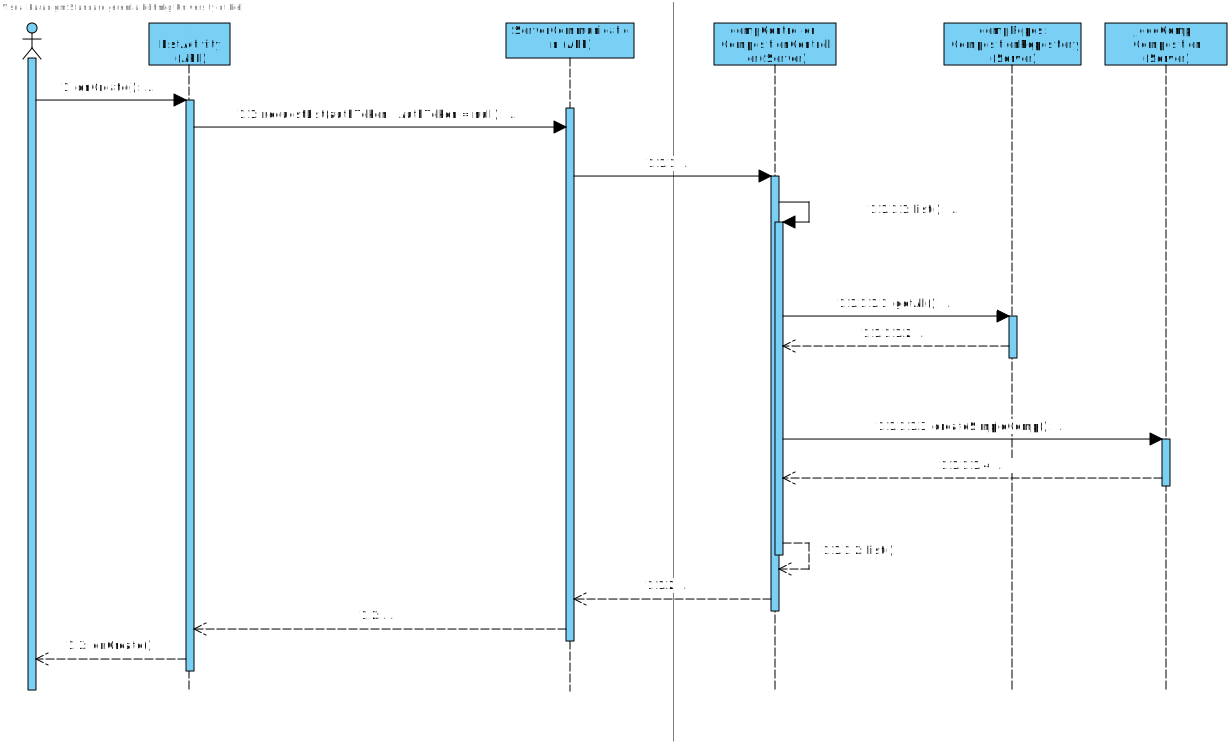
\includegraphics[width=\textwidth]{img/Diagramme/Sequenz/Overview}
	\caption{Sequenzdiagramm}
	\label{fig:sequenz-overview}
\end{figure}
\noindent
Zusammengefasst beschreibt dieses Diagramm das grobe Verhalten des Systems, das abläuft, wenn ein Nutzer über die App sich die für ihn anzeigbaren Kompositionen auflisten lässt. Dabei bezieht es die Kommunikation zwischen Android App und Backend mit ein.\newline

\noindent Der Benutzer öffnet die App, wodurch die Methode onCreate() der ListActivity aufgerufen wird. Beim Start sendet die App ein HTTPS-Request an den Server. Daraufhin fragt der Server die Daten aus der Datenbank ab und erstellt aus diesen ein versendbares Objekt in Form einer Liste von SimpleComp-Objekten. Diese schickt das Backend im Rahmen der Antwort auf den GET-Request an die App, welche die erhaltenen Daten verarbeitet, worauf sie diese dem Benutzer anzeigen kann.

\section*{Sequenzdiagramme der App}
\subsection*{ Öffnen der ListActivity}

\begin{figure}[h]
	\centering
	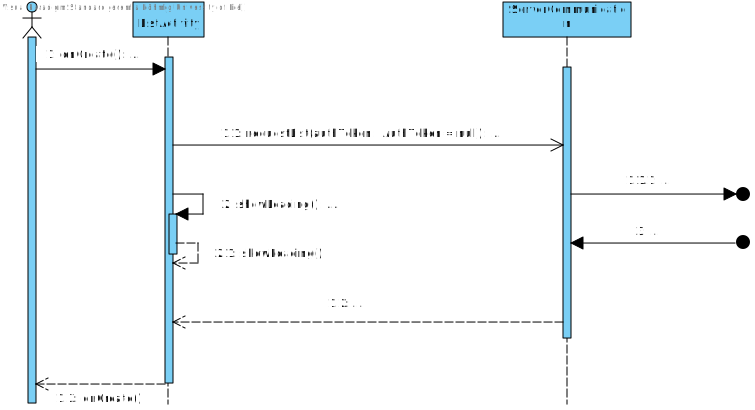
\includegraphics[width=\textwidth]{img/Diagramme/Sequenz/App_list}
	\caption{Sequenzdiagramm - Öffnen der ListActivity}
	\label{fig:sequenz-app_list}
\end{figure}
\noindent
Dieses Sequenzdiagramm zeigt den Vorgang, der abläuft, wenn die ListActivity initial gestartet wird und mit einer Liste aus Kompositionseinträgen zu füllen ist.\newline

\noindent Der Ablauf der Aktivitäten beginnt mit dem Start der ListActivity, bei dem ein Rufen der Standard-Methode onCreate() erfolgt. Da der Nutzer noch nicht eingeloggt ist, startet die App eine requestList()-Anfrage ohne Token. Diese läuft in einem eigenen Thread, damit der UI-Thread nicht blockiert. Die Methode requestList() führt einen HTTPS-Request an das Backend aus. In der Zeit, in der die ListActivity die Antwort noch nicht erhalten hat, zeigt sie mithilfe von showLoading() eine Ladeanimation an.
\pagebreak
\subsection*{ Klicken auf Kompositionseintrag}

\begin{figure}[h]
	\centering
	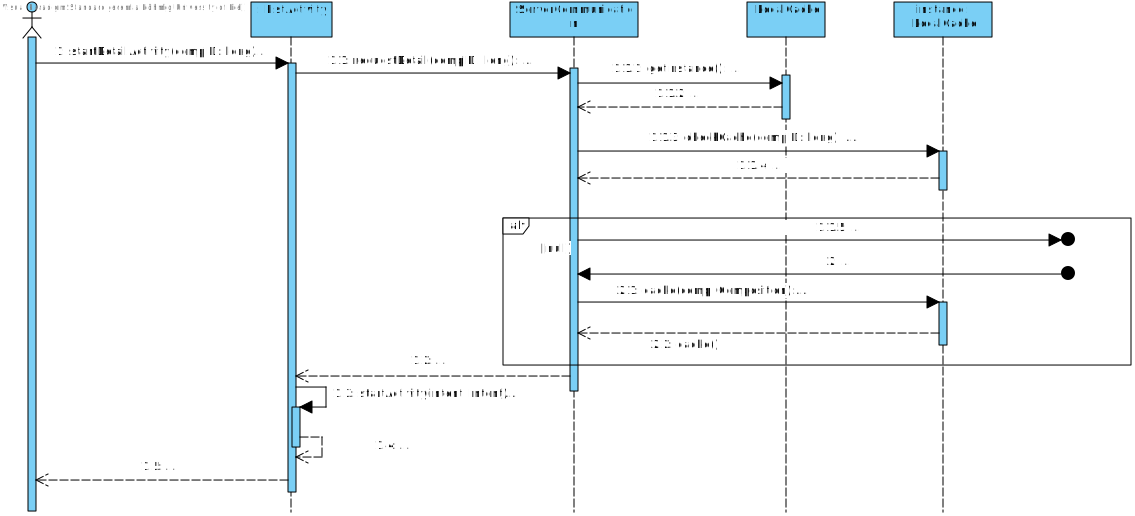
\includegraphics[width=\textwidth]{img/Diagramme/Sequenz/App_detail}
	\caption{Sequenzdiagramm - Klick auf Kompositionseintrag}
	\label{fig:sequenz-App_detail}
\end{figure}


\noindent Fortführend schließt sich dieses Sequenzdiagramm an den Usage-Flow des obigen an. Ist die Liste geladen, will der Nutzer sich früher oder später eine der Kompositionen  detailliert als Grafik anzeigen lassen. Hierfür reicht ein Tippen auf das jeweilige Listenelement aus, um die Detailansicht in Form der DetailActivity aufzurufen.\newline
\\
Durch die genannte UI-Aktion wird die Methode startDetailActivity() aufgerufen, was die statische Methode requestDetail() veranlasst, im LokalCache nach der gewünschten Komposition zu suchen.
Falls diese noch nicht im Cache ist, sendet die App eine HTTPS-Request an den Server.
In der Antwort auf diesen Request sind alle nötigen Details der Komposition enthalten, wozu unter anderem ihre Nodes zählen.
Die Details werden in der Komposition gespeichert, die wiederum im LokalCache abgelegt ist, und so auch an die ListActivity zurückgegeben. Diese übergibt die nun mit Details ausgestattete Komposition an einen Intent, der zum Starten der DetailsActivity dient.\newline
\\
Da LocalCache ein Singleton ist, muss man zu Beginn die Instanz abrufen. Wir planen, die Instanz vorzudefinieren (eager instantiation), wodurch der Fall, dass man die Instanz erst erzeugen müsste, nie eintritt.\newline
\\ \noindent
Die Methode httpsRequest() wird nicht implementiert, sondern dient hier zur Abstraktion. In der Implementation wird diese Abfrage asynchron erfolgen und in einem anderen Thread laufen, so dass sie den UI-Thread nicht blockiert. 


\pagebreak
\section*{Sequenzdiagramme des Servers}


\begin{figure}[h]
	\centering
	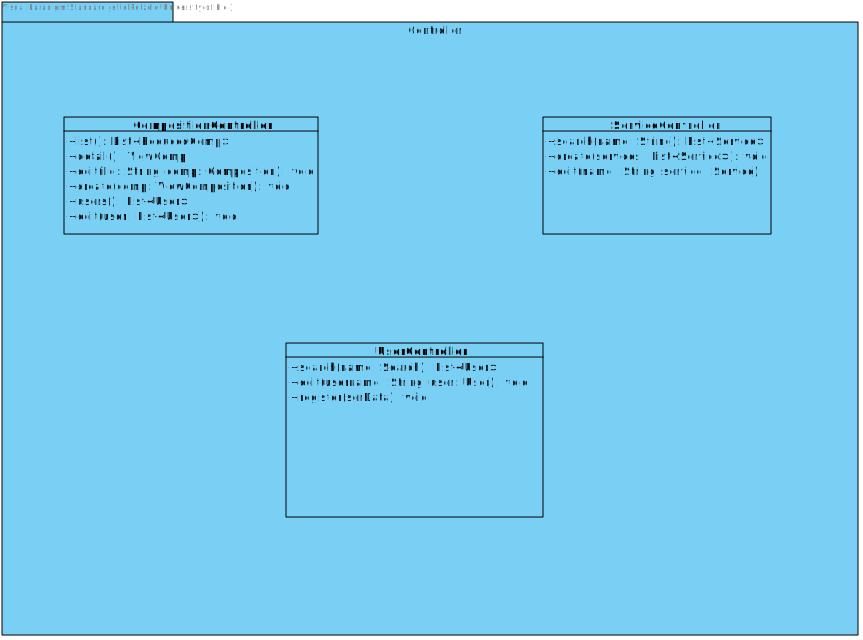
\includegraphics[width=\textwidth]{img/Diagramme/Sequenz/Controller}	
	\caption{Sequenzdiagramm - Kompositionsanfrage}
	\label{fig:sequenz-a}
\end{figure}
\noindent
Nach der Betrachtung der Android-App folgt nun eine detailliertere Darstellung, wie sich die Server-Seite verhält, wenn eine Komposition in Detailansicht angefragt wird.\\ \\ 
\noindent Eine solche Anfrage wird vom CompositionsController entgegengenommen.
Die angefragte Komposition wird in der Datenbank nachgeschlagen (über das CompositionRepository) und als Composition-Objekt zurückgegeben.
Anschließend wird eine DetailComp erstellt, welche die benötigten Daten für das Frontend enthält. 
Um diese zu erstellen, müssen zunächst alle CompositionNodes und danach alle CompositionEdges in versendbare Objekte (Nodes und Edges) umgewandelt werden. 
Dabei wird für jede Kante noch die Kompatibilität überprüft und mögliche Alternativen werden gesucht und ggf. gespeichert. Zurückgeliefert wird also eine DetailComp, die in allen Kanten eine CompatibilityAnswer enthält.\newline
\\ \noindent
Wir haben uns dafür entschieden, eine Util-Klasse zur Berechnung der Compatibility zwischen zwei verschiedenen Diensten (repräsentiert durch ihre IDs) zu verwenden.
Da auch HTTPS-Requests erwartet werden, die nur zu zwei einzelnen Diensten die Kompatibilität erfahren wollen, wäre eine Implementierung dieser Funktion in der Edge-Klasse nicht praktikabel.\newline
\\ \noindent
Da es sich bei dem durch dieses Sequenzdiagramm modellierten dynamischen Verhalten um das komplexeste unseres Backends handelt und sich viele andere Abläufe in ihm widerspiegeln, sei nur dieses als Repräsentant der Arbeitsweise aufgeführt.

\newpage
\section*{Sequenzdiagramme des Web Frontends}
\subsection*{ Erstellen einer Komposition}

\begin{figure}[!h]
	\centering
	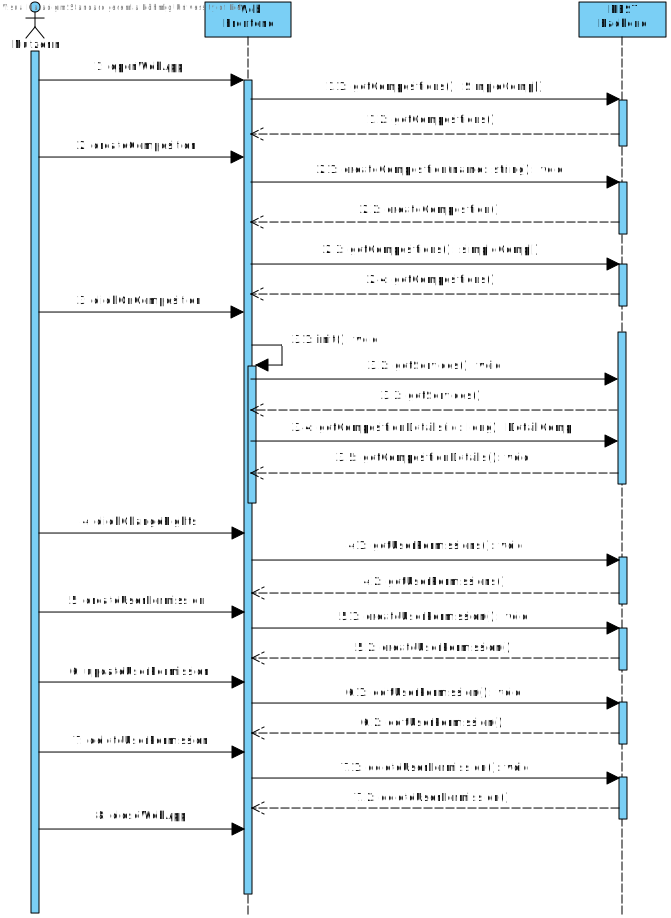
\includegraphics[width=.5\textwidth]{img/Diagramme/Sequenz/Frontend_createComp}
			
	\caption{Sequenzdiagramm - Erstellen einer Komposition}
	\label{fig:sequenz-createComp}
\end{figure}

\noindent
Um eine neue Komposition zu erstellen, fragt das Web Frontend zunächst die dem Nutzer verfügbaren Kompositionen vom Backend an und stellt diese bei Erhalt der Antwort dar. Über ein Eingabefeld lässt sich ein Name für eine neue Komposition festlegen und mit einem zusätzlichen Knopf erstellen. Hiernach wird die Liste der verfügbaren Kompositionen aktualisiert. Ein Klick auf die Komposition löst das Abrufen der bisher nicht erhaltenden Kompositionsdetails vom Backend aus. Erhält das Frontend diese, zeigt es sie in der Bearbeitungsansicht an. Als Autor der Komposition lassen sich nun die Listen mit den Nutzenden einsehen und bearbeiten, die diese Komposition betrachten oder bearbeiten dürfen. Hierbei fordert das Web Frontend alle Informationen immer aus dem Backend an, beziehungsweise schickt Aktualisierungen vom Nutzenden an das Backend.

\newpage
\subsection*{ Bearbeiten einer Komposition}

\begin{figure}[!h]
	\centering
	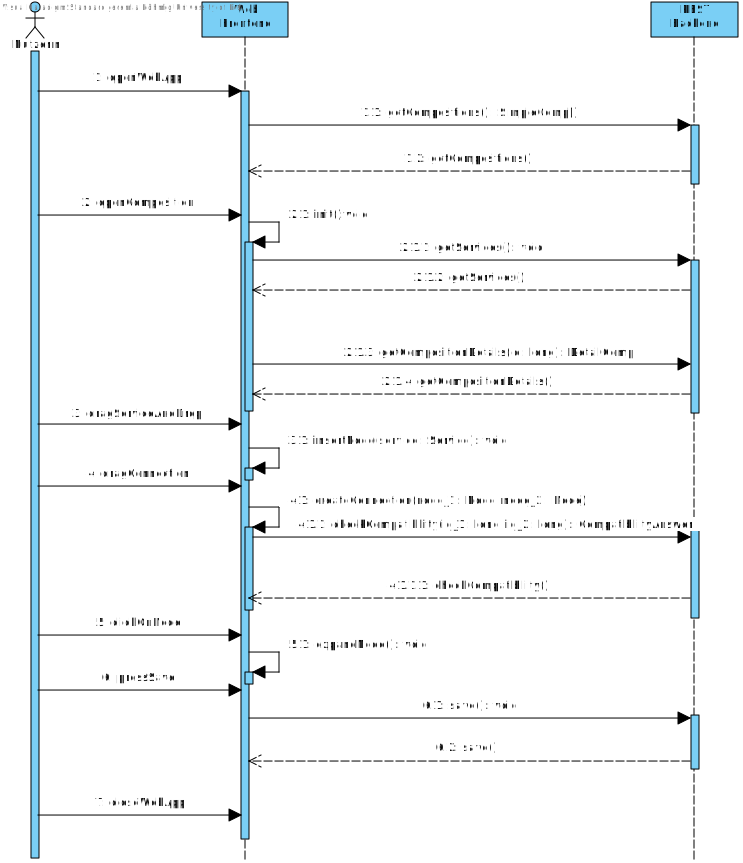
\includegraphics[width=.5\textwidth]{img/Diagramme/Sequenz/Frontend_editComp}			
	\caption{Sequenzdiagramm - Bearbeiten einer Komposition}
	\label{fig:sequenz-editComp}
\end{figure}
\noindent
Um eine Komposition zu bearbeiten, fragt das Frontend zunächst wieder die dem Nutzer verfügbaren Kompositionen vom Backend an und stellt diese dar. Ein Klick auf die Komposition lässt die Details sowie Services vom Backend abrufen und in der Bearbeitungsansicht anzeigen. Indem man einen Service aus dem SidePanel in das Canvas zieht, erstellt man lokal einen Knoten. Das Verbinden von zwei Knoten erstellt zunächst lokal eine Verbindung, wobei eine Anfrage an das Backend geht, die das Überprüfen der Kompatibilität überprüfen lässt. Beim Klicken auf einen Knoten wird eine Detailansicht für den verwendeten Dienst angezeigt. Wiederum sendet ein Klick auf Speichern die aktualisierte Komposition an den Server.

\newpage
\subsection*{ Bedienung des Adminpanels}

\begin{figure}[!h]
	\centering
	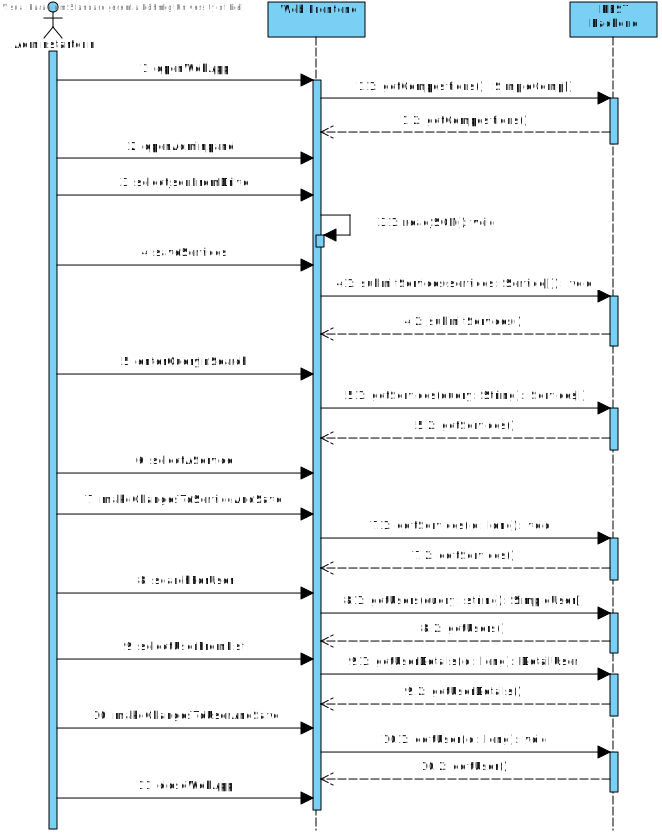
\includegraphics[width=.5\textwidth]{img/Diagramme/Sequenz/Frontend_admin}			
	\caption{Sequenzdiagramm - Bedienung des Adminpanels}
	\label{fig:sequenz-adminPanel}
\end{figure}
\noindent
Das Adminpanel lässt sich aus der Kompositionsübersicht erreichen. Über eine Maske lässt sich eine JSON-Datei mit Services einlesen, die zunächst nur lokal zwischengespeichert und dann bei Bestätigung an das Backend übermittelt werden. Ein Suchfeld für Dienste erlaubt, eine Suchanfrage an das Backend zu schicken und durch Auswählen eines Listeneintrags die Details eines Services zu bearbeiten, die das Frontend bei Bestätigung der Eingabe an das Backend übermittelt. Weiterhin ermöglicht das Frontend die Suche nach registrierten Nutzenden. Wiederum fragt das Auswählen eines Nutzers die Details vom Backend ab, die ein Administrierender bearbeiten kann. Nach Bestätigung der Änderungen sendet das Frontend die angepassten Daten an das Backend, welches sie speichert.


	\chapter{Glossar}\label{chp:glossar}
	\thispagestyle{fancy}
	\begin{tcolorbox}
In diesem Glossar können Akronyme und abkürzende Schreibweisen aufgelistet werden. 
Alle verwendeten Abkürzungen innerhalb des Projekts müssen hier erläutert werden.
\end{tcolorbox}

\begin{table}[h]
	\centering
	\begin{tabularx}{\textwidth}{X X}
		\rowcolor[HTML]{C0C0C0} 
		\textbf{Abkürzung} & \textbf{Beschreibung} \\
		Abk. A & Beschreibung A \\
		\rowcolor[HTML]{E7E7E7} 
		Abk. B & Beschreibung B \\
		Abk. C & Beschreibung C \\
		\rowcolor[HTML]{E7E7E7} 
		Abk. D & Beschreibung D \\
		Abk. E & Beschreibung E \\
		\rowcolor[HTML]{E7E7E7} 
		Abk. F & Beschreibung F \\
		Abk. G & Beschreibung G
	\end{tabularx}
	\caption{Glossar}
	\label{table:glossar}
\end{table}

	\bibliography{references}
	\pagenumbering{gobble} % Nummerierung deaktivieren

\end{document}
